\chapter{Applications} \label{chap:App}
\thispagestyle{empty}

\section{Risks Measures}

In this section we discuss different ways of measuring the risk of a portfolio.
\begin{definition}
	A portfolio with $n$ assets, $A_1, A_2, \dots, A_n$, is a vector $x^\top = (x_1, x_2, \dots, x_n)\in \R^n$, each coordinate $x_i$ being the weight of the capital invested in asset $A_i$.
\end{definition}

In financial science, Risk is the probability of losing capital. Considering the loss as a random variable, we may calculate the standard deviation (volatility) of its distribution. Nobel laureate in economics, Harry Markowitz in 1952 (see \cite{Markowitz1952}) assumed that volatility to be modelled by a normal distribution.


Other risk measures are expressed in terms of loss distribution percentiles. An upper percentile of the loss distribution is called \textit{Value-at-Risk} (here $\mbox{VaR}_\beta$)\footnote{$\mbox{VaR}_\beta$ is the percentile of the loss distribution.}. For instance, with probability $95\%$, the loss is less than $\mbox{VaR}_{0.95}$. The popularity of $\mbox{VaR}_\beta$ is mostly related to being a simple way to understand high loss representations. $\mbox{VaR}_\beta$ may be estimated and managed quite efficiently, when the underlying risk factors are normally (log-normally) distributed.

An alternative risk measure of is known as the \textit{Conditional Value-at-Risk} ($\mbox{CVaR}_\beta$)\footnote{$\mbox{CVaR}_\beta$ is the average loss in the $100(1-\beta)$\% worst case scenarios.}. The $\mbox{CVaR}_\beta$ risk measure is closely related to $\mbox{VaR}_\beta$. For continuous distributions, $\mbox{CVaR}_\beta$ is defined as the conditional expected loss, under the condition that it exceeds $\mbox{VaR}_\beta$, see Rockafellar and Uryasev (see \cite{RockafellarUryasev2001}). For continuous distributions, this risk measure is also known as \emph{Expected Shortfall}, \textit{Mean Excess Loss}, \textit{Mean Shortfall}, or \textit{Tail Value-at-Risk}.


\begin{figure}[!ht]
	\centering
	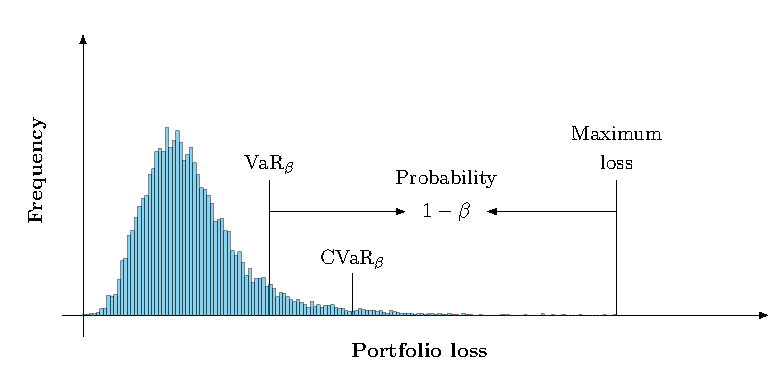
\includegraphics{figures/VarCvar.pdf}
	\caption{Portfolio Loss Distribution, VaR and CVaR.}
	\label{fig:VarCvar}
\end{figure}

\begin{remark}\normalfont\label{re:Normal}

	Since loss may be seen as negative return, if the loss distribution of a portfolio $x$ is normal, it follows that both $\mbox{VaR}_\beta$ and $\mbox{CVaR}_\beta$ may be rewritten by
	\[
		-\mu(x)+c\sigma(x)
	\]
	where $\mu(x)$ and $\sigma(x)$ denote the return mean value and volatility,  associated with portfolio $x$, and $c$ is a constant (see \cite[Chapter 2]{Roncalli2014}). If the portfolio manager has very optimistic forecasts, component $\mu(x)$ may reduce the risk measure substantially. This explains why omitting the mean component has been adopted as a standard practice by the asset management industry.
\end{remark}
% \begin{example}\normalfont
% 	We consider three stocks $A$, $B$ and $C$ whose current prices are respectively $\$ 15.00$, $\$ 25.00$ and $\$ 30.00$. We assume that their expected returns equals $30$ bps\footnote{1 bps or one basis point is equivalent to
% 		0.01\% (the hundredth part of 1\%) or 0.0001 in decimal form.}, $50$ bps and $20$ bps on a daily basis and their daily volatilities are $3\%$, $2\%$, and $1\%$ respectively. The asset correlation matrix is given by
% 	\[
% 		\rho = \left(
% 		\begin{array}{rrr}
% 				1.00 & 0.40 & 0.15 \\
% 				0.40 & 1.00 & 0.60 \\
% 				0.15 & 0.60 & 1.00
% 			\end{array}
% 		\right)
% 	\]

% 	We consider a portfolio composed by $100$ stocks $A$, $200$ stocks $B$ and $100$ stocks $C$. The value of this portfolio is $\$ 9,500.00$, being $\$ 1,500.00$ invested in stock $A$, $\$ 5,000.00$ in stock $B$ and $\$ 3,000.00$ in stock $C$, therefore the weights of the stocks in this portfolio are $15.79\%$, $52.63\%$, and $31.58\%$ respectively, so $x=(0.1579;\;0.5263;\; 0.3158)$. The expected loss of the portfolio is $\mu(x) = -30\times0.1579+50\times0.5263+20\times0.3158$, that is, $\mu(x) = -37$ bps. Using the relationship $\Sigma_{i,j}=\rho_{i,j}\sigma_1\sigma_j$ we find the covariance matrix
% 	\[
% 		\Sigma = \left(
% 		\begin{array}{llr}
% 				9.0 & 2.4 & 4.5 \\
% 				2.4 & 4.0 & 1.2 \\
% 				4.5 & 1.2 & 1.0
% 			\end{array}
% 		\right)\times10^{-4},
% 	\] since the volatility of portfolio is given by $\sigma^2(x) = x^\top \Sigma x$, we have that $\sigma(x) = 1.51\%$.

% 	Considering $\alpha = 0.99$, we have $\Phi^{-1}(0.99) = 2.325$ and
% 	$\phi(\Phi^{-1}(0.99))=\phi(2.325)=2.68\%$. Using the equations
% 	$(\ref{eq:var2})$ and $(\ref{eq:cvar2})$ we have

% 	\[
% 		\begin{aligned}
% 			\mathrm{VaR}_{99\%}(x) & = -0.37\% + 2.325 \times 1.51\% = 3.14\%              \\
% 			\mathrm{ES}_{99\%}(x)  & = -0.37\% + \frac{2.68}{0.01} \times 1.51\% = 3.68\%.
% 		\end{aligned}
% 	\]

% 	Risk can also be expressed in monetary terms, in this case,

% 	\[
% 		\begin{aligned}
% 			\mathrm{VaR}_{99\%}(x) & = 3.14\% \times \$ 9,500.00 = \$ 298.30  \\
% 			\mathrm{ES}_{99\%}(x)  & = 3.68\% \times \$ 9,500.00 = \$ 349.60.
% 		\end{aligned}
% 	\]
% 	According to the result of {\rm VaR}, in $99\%$ of the days, the loss will be less than $\$ 298.30$, however in the $1\%$ of the remaining days the {\rm VaR} does not measure how much great can be the loss, this is the role of {\rm CVaR} which indicates that the average loss will be $\$ 349.60$ on the worst $1\%$ days.
% \end{example}


\section{Portfolio optimization}

In this section we present some ways to build a portfolio. In a universe of $n$ assets let $x^\top = (x_1, x_2, \dots, x_n)$ be a portfolio and by $R_i$ denote the return of asset $i$. If $R^\top=(R_1, R_2, \dots, R_n)$  is the random vector of assets, then the return of the portfolio $x$ is given by:
\[
	R(x) = x_1R_1+x_2R_2+\cdots x_nR_n = x^\top R.
\]
If we denote by $\mu$ and $\Sigma$ the vector of expected returns and the covariance matrix of asset returns respectively, we deduce that the expected return of portfolio $x$ equals:
\[
	\mu(x) = x^\top \mu.
\]
Its variance is given by:
\[
	\sigma^2(x) = x^\top \Sigma x.
\]
The mean-variance portfolio (MVP) of Markowitz (see \cite{Markowitz1952}), consists of maximizing the expected return $\mu(x)$ for a fixed value $\nu$ of the volatility $\sigma(x)$, achieved by solving the problem:
\begin{eqnarray}\label{prob:MVP}
	\min_{x} \, \{- \mu(x)\}, \\
	\mbox{s.t. }\left\{
	\begin{aligned}\nonumber
		\sigma^2(x) = \nu,  & \\
		\mathbf{1}^\top x=1 &
	\end{aligned}
	\right.
\end{eqnarray}
where $\textbf{1}^\top =(1,1,\dots,1)$. The condition $\mathbf{1}^\top x=1$ means that the capital is fully invested.

A portfolio optimization  problem is defined when we want to minimize (or maximize) a performance measure subject to a set of constraints. Here are some examples of performance measures and constraints:

\begin{itemize}
	\item \textbf{Performance Measures}
	      \begin{itemize}
		      \item Expected return: $\mu(x)$;
		      \item Volatility: $\sigma(x)$;
		      \item Sharpe Ratio (SR): expected return per unit of risk
		            \[
			            \mbox{SR}(x) = \frac{x^\top \mu - r_f}{\sigma(x)}
		            \]
		            where $r_f$ is the risk-free rate (e.g. treasury bill interest rate);
		      \item Information Ratio (IR): Sharpe Ratio with $r_f=0$;
		      \item $\mbox{VaR}_\beta$ (Value at Risk): loss quantile;
		      \item $\mbox{CVaR}_\beta$ (Conditional Value at Risk): expected loss value above $\mbox{VaR}_\beta$.
	      \end{itemize}
\end{itemize}

\begin{itemize}
	\item \textbf{Constraints}
	      \begin{itemize}
		      \item Capital constraint: $\textbf{1}^\top x=1$;
		      \item Long-only constraint: $x\geq0$;
		      \item Self-financial constraint: $\textbf{1}^\top x=0$;
		      \item Holding constraint: $\mathbf{I}\leq x\leq \mathbf{J}$ where $\mathbf{I},\mathbf{J}\in\R^n$ are lower and upper portfolio bounds.
		      \item Leverage constraint: $\|x\|_1\leq K$.
	      \end{itemize}
\end{itemize}

Some known portfolio optimization problems are:

\noindent\textbf{Minimum Variance Portfolio (MVP)}

Minimize variance with fully invested capital
\begin{eqnarray}\label{eq:MVP}
	\min_{x} \,\big\{x^\top \Sigma x\big\}, \\
	\mbox{s.t. }\left\{
	\begin{aligned}
		\mathbf{1}^\top x=1 \\
	\end{aligned}
	\right\}.\nonumber
\end{eqnarray}

\noindent\textbf{Maximum Sharpe Ratio Portfolio (MSRP)}

Maximize Sharpe ratio with self-financial constraints
\begin{eqnarray*}
	\max_{x} \,\big\{\mbox{SR}(x)\big\}, \\
	\mbox{s.t. }\left\{
	\begin{aligned}\nonumber
		\mathbf{1}^\top x=0, & \\
		\|x\|_1\leq K,
	\end{aligned}
	\right.
\end{eqnarray*}
the latter constraint being a leverage restriction. Performances and constraints may also be combine as
\begin{eqnarray*}
	\min_{x} \,\big\{\lambda \mbox{CVaR}_\beta(x) - \mu(x)\big\}, \\
	\mbox{s.t. }\left\{
	\begin{aligned}\nonumber
		\mathbf{1}^\top x=1, & \\
		\|x\|_1\leq K.
	\end{aligned}
	\right.
\end{eqnarray*}
Here, $\lambda$ is a parameter controlling the investor risk-aversity.

Furthermore, we may consider portfolio optimization problems as multi-objective problems: Let $f:\R^n\to\R^2$ be the function $f(x)= \big(\mathcal{P}(x), \mathcal{R}(x)\big)$, where $\mathcal{P}(x)$ is a performance measure (that we want to minimize) of portfolio $x$ and $\mathcal{R}(x)$ is a risk measure of $x$. We want to solve the problem
\begin{eqnarray*}
	\min_{x} \,\Big\{f(x)= \big(\mathcal{P}(x), \mathcal{R}(x)\big)\Big\}, \\
	\mbox{s.t. }\left\{
	\begin{aligned}\nonumber
		\mathbf{1}^\top x=1.
	\end{aligned}
	\right.
\end{eqnarray*}

In all these problems we want to optimize a performance measure. In the remainder of this chapter we present a new approach with a risk allocation perspective.


\section{Risk Parity}

Markowitz’s portfolio was never fully embraced by practitioners, among other reasons since, considers only the overall risk of the portfolio, disregarding diversification risks (i.e., concentrates too much risk in few assets, as observed during the 2008 financial crisis). In order to avoid this problem, one solution are to consider the risk parity portfolio.

Risk parity is an approach to portfolio management that focuses on risk, rather than capital allocation. The risk parity approach asserts that, when asset allocations are adjusted to the same risk level, the portfolio may achieve a higher Sharpe ratio as well as being more resistant to market downturns.

While the minimum variance portfolio  (MVP) tries to minimize the variance (with the disadvantage the portfolio risk may be concentrated in only a few assets), the risk parity portfolio distributes the weights, so that the risk contributions of all assets (or asset class, such as bonds, stocks, real estate, etc.) are the same.

In order to define a risk-based allocation strategy, it is necessary to define how the risk of each asset affects the overall risk of the portfolio.
Let $x^\top=(x_1,x_2,\dots,x_n)$ be a portfolio with $n$ assets and $\mathcal{R}(x)$ be a differentiable, homogeneous risk measure of $x$. We have
\[
	\mathcal{R}(x)=\frac{d}{d\lambda}\mathcal{R}(\lambda x)=\sum_{i=1}^n x_i \frac{\partial \mathcal{R} (x)}{\partial x_i}.
\]
We define the risk contribution of asset $i$  by
\[
	\mathcal{RC}_i(x)= x_i \frac{\partial \mathcal{R}(x)}{\partial x_i}.
\]
Therefore, the risk may be written as follows
\[
	\mathcal{R}(x)=\sum_{i=1}^n \mathcal{RC}_i(x)
\]
which is known as \textbf{Euler's Allocation Principle}.

The volatility as well as $\mbox{CVaR}_\beta$  satisfies the properties required by the risk measure, $\mathcal{R}$, defined above. However, $\mbox{VaR}_\beta$ satisfies these properties only in the Gaussian case. When asset returns follows a Normal Distribution, by Remark \ref{re:Normal}, we have that
$\mathcal{R}(x)=\sigma(x)=\sqrt{x^\top\Sigma x}$, it follows that
\[
	\mathcal{RC}_i(x)= x_i \frac{\partial \sigma(x)}{\partial x_i}=\frac{x_i (\Sigma x)_i}{\sqrt{x^\top\Sigma x }}.
\]

It may be interesting for the investor to choose different risk levels for different assets. In this case the investor choose the percentage of risk, $b_i$, that each asset should have in the portfolio, that is,
\begin{equation}\label{eq:RBP}
	\mathcal{RC}_i(x)=b_i\mathcal{R}(x),
\end{equation}
$b_i\geq 0$ for all $i$, and
${\bf 1}^\top b =1$, with $b^\top=(b_1, b_2, \dots, b_n)$. A portfolio distribution based on equation \eqref{eq:RBP} is called a \textit{risk budgeting portfolio} (RBP). When $b_i=1/n$, for all $i$, the distribution is called \textit{risk parity portfolio} (RPP) or \textit{equal risk portfolio} (ERP).

In general, find the risk budgeting portfolio consists in solving the following non-linear system
\begin{eqnarray*}
	\mathcal{RC}_i(x)=b_i\mathcal{R}(x), \\
	\mbox{s.t. }\left\{
	\begin{aligned}\nonumber
		b_i \geq 0,        \\
		x_i \geq 0,        \\
		{\bf 1}^\top b =1, \\
		{\bf 1}^\top x =1.
	\end{aligned}
	\right.
\end{eqnarray*}

In 2012, Kaya and Lee (see \cite{KayaLee2012}) show that, in the Gaussian case, the risk budgeting portfolio may be found solving the optimization problem
\begin{eqnarray}
	\min_{x\geq \textbf{0}}\, \{-b^\top \ln(x)\}; \label{eq:RPP}\\
	\mbox{s.t. }\left\{ \nonumber
	\begin{aligned}\nonumber
		\sigma^2(x)\leq \sigma_0, \\
		{\bf 1}^\top x =1,
	\end{aligned}
	\right.
\end{eqnarray}
$\sigma_0$ being a volatility target.


\section{A Backtest Study}

In this section we present a backtest study of a portfolio build with the 10 biggest companies on the brazilian market: Ambev S.A. (ABEV3), B3 S.A. (B3SA3), Banco do Brasil S.A. (BBAS3), Banco Bradesco S.A. (BBDC4), Itaúsa S.A. (ITSA3), Itaú Unibanco S.A. (ITUB4), Lojas Renner S.A. (LREN3), Petróleo Brasileiro S.A (PETR4), Vale S.A. (VALE3) and WEG S.A. (WEGE3), in parentheses we have the tickers of each company.  We did a backtest, building 2 portfolios with monthly rebalance. One was the minimum variance portfolio (MVP), and the other the risk parity portfolio (RPP),  obtained solving optimization problems \eqref{eq:MVP} and \eqref{eq:RPP}, respectively. Data pertaining to the period between January 2016  and June 2022, was taken from Yahoo Finance (\url{http://finance.yahoo.com}). For rebalancing, the volatilities were calculated using data from the previous 12 months. 2016 year data was used only for past volatilities calculations.

Generally, MVP is rarely used in practice, one of the reasons resides in the fact that the weights (and consequently the risks), may be concentrated in a few assets. Figure \ref{fig:totalRiskMVP} shows the weight distribution as well as the risk contribution of stocks during the MVP backtest study. We note that the MVP concentrates capital in few assets and consequently also concentrates risk in these assets.

% \begin{figure}[H]
% 	%\begin{adjustwidth}{2.2cm}{2.2cm}
% 	\begin{subfigmatrix}{3}
% 		\subfigure[January]{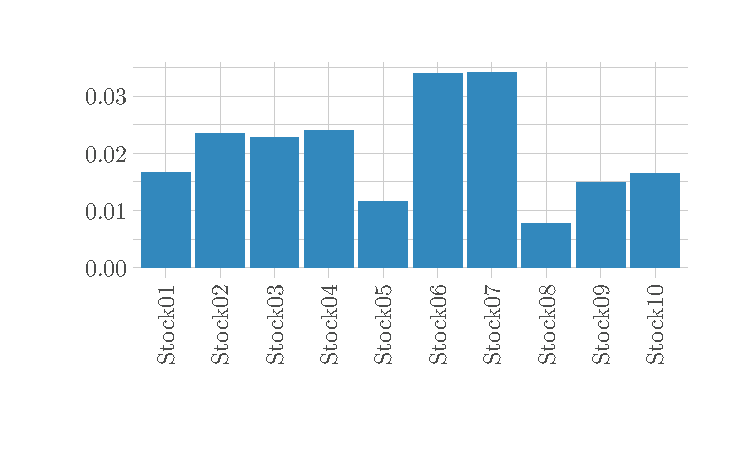
\includegraphics{figures/RiskContribEqual101.pdf}}
% 		\subfigure[February]{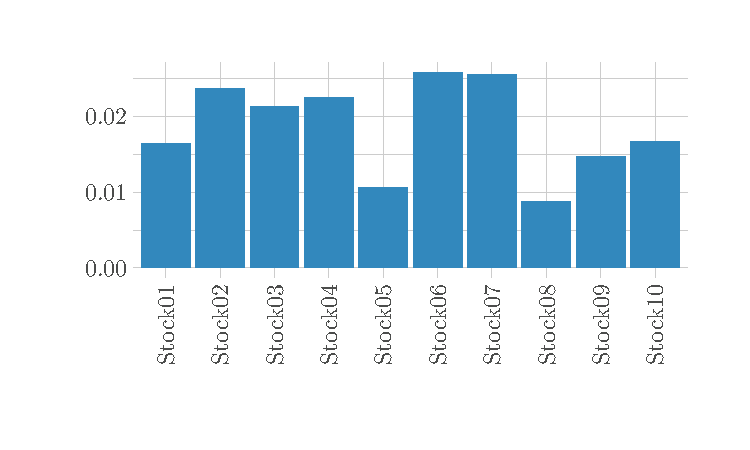
\includegraphics{figures/RiskContribEqual102.pdf}}
% 		\subfigure[March]{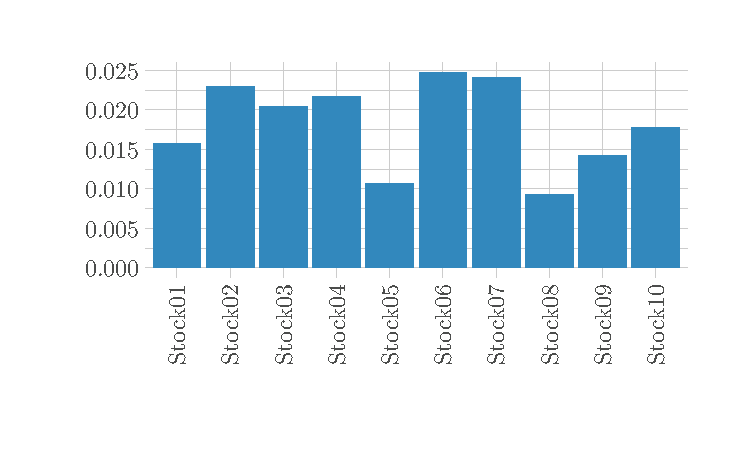
\includegraphics{figures/RiskContribEqual103.pdf}}
% 		\subfigure[April]{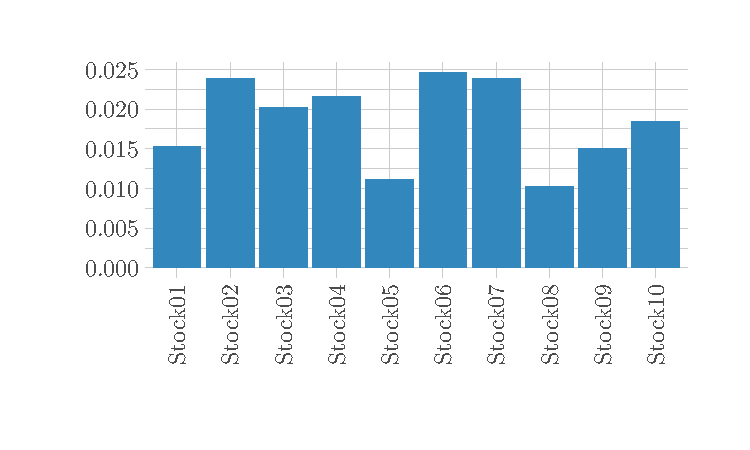
\includegraphics{figures/RiskContribEqual104.pdf}}
% 		\subfigure[May]{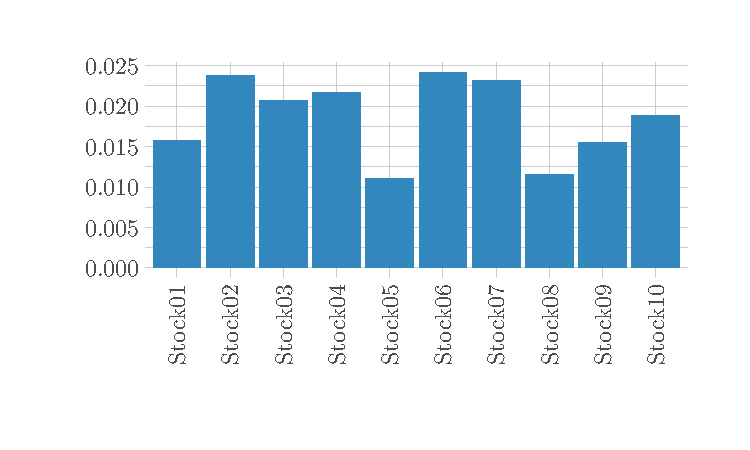
\includegraphics{figures/RiskContribEqual105.pdf}}{}
% 		\subfigure[June]{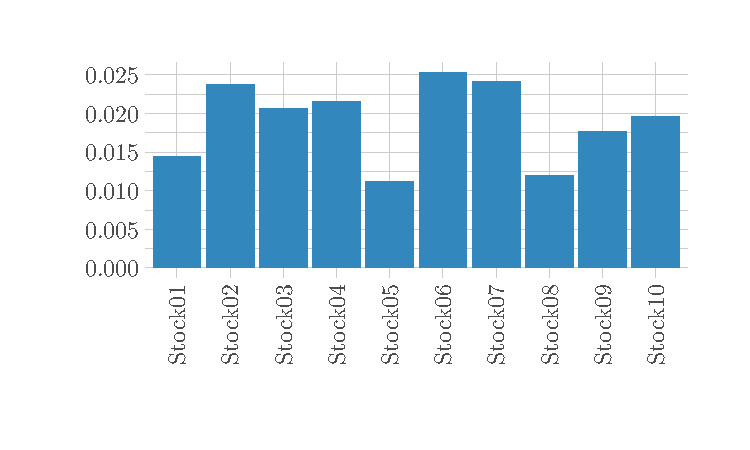
\includegraphics{figures/RiskContribEqual106.pdf}}
% 	\end{subfigmatrix}
% 	\caption{Risk Contributions of EWP.}
% 	\label{fig:condProj1}
% 	%\end{adjustwidth}
% \end{figure}


% \begin{figure}[H]
% 	%\begin{adjustwidth}{2.2cm}{2.2cm}
% 	\begin{subfigmatrix}{3}
% 		\subfigure[January]{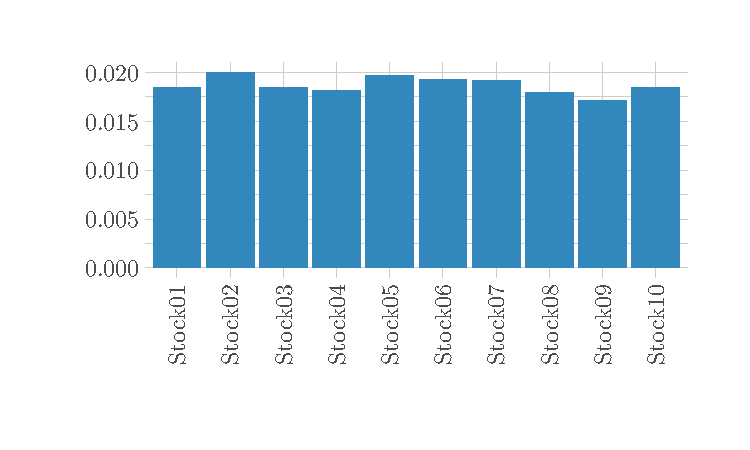
\includegraphics{figures/RiskContrib101.pdf}}
% 		\subfigure[February]{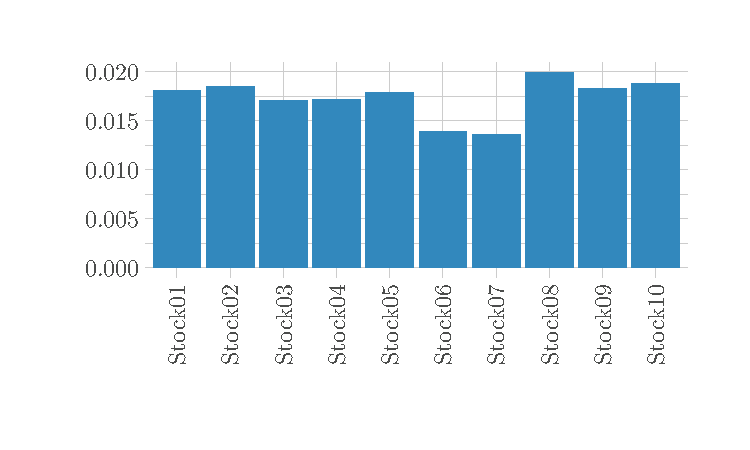
\includegraphics{figures/RiskContrib102.pdf}}
% 		\subfigure[March]{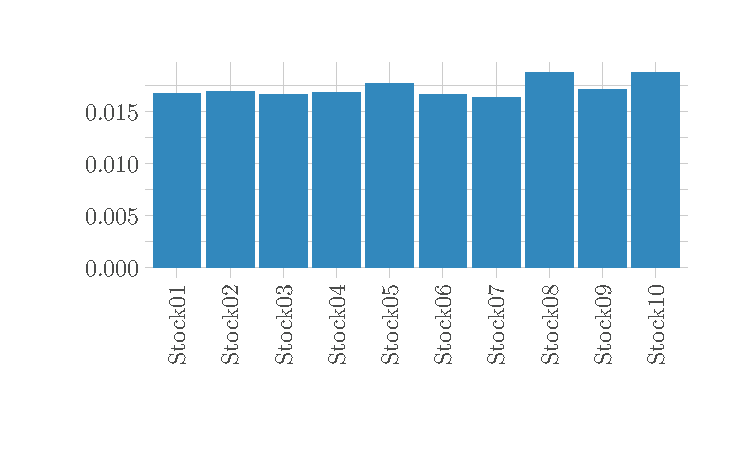
\includegraphics{figures/RiskContrib103.pdf}}
% 		\subfigure[April]{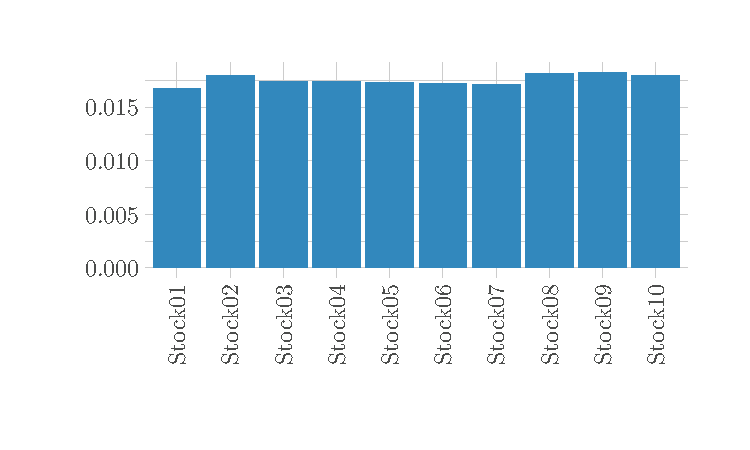
\includegraphics{figures/RiskContrib104.pdf}}
% 		\subfigure[May]{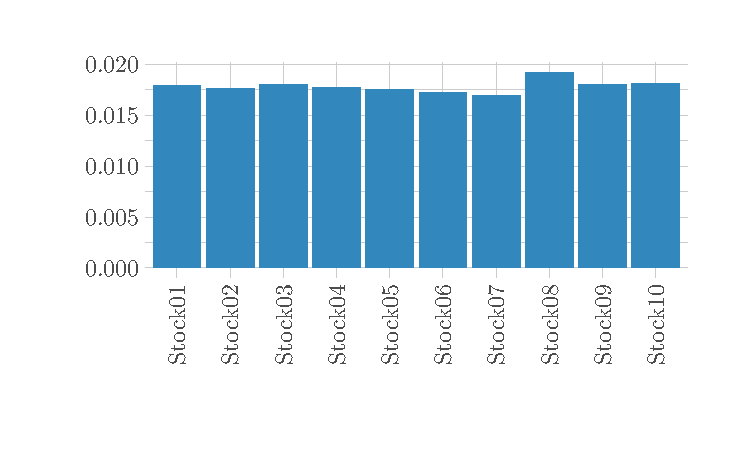
\includegraphics{figures/RiskContrib105.pdf}}
% 		\subfigure[June]{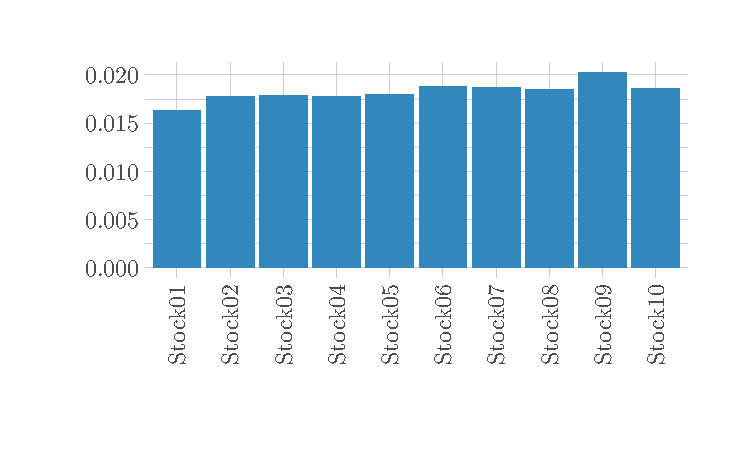
\includegraphics{figures/RiskContrib106.pdf}}
% 	\end{subfigmatrix}
% 	\caption{Risk Contributions of RPP.}
% 	\label{fig:condProj1}
% 	%\end{adjustwidth}
% \end{figure}


\begin{figure}[H]
	%\begin{adjustwidth}{2.2cm}{2.2cm}
	\begin{subfigmatrix}{2}
		\subfigure[Weigths]{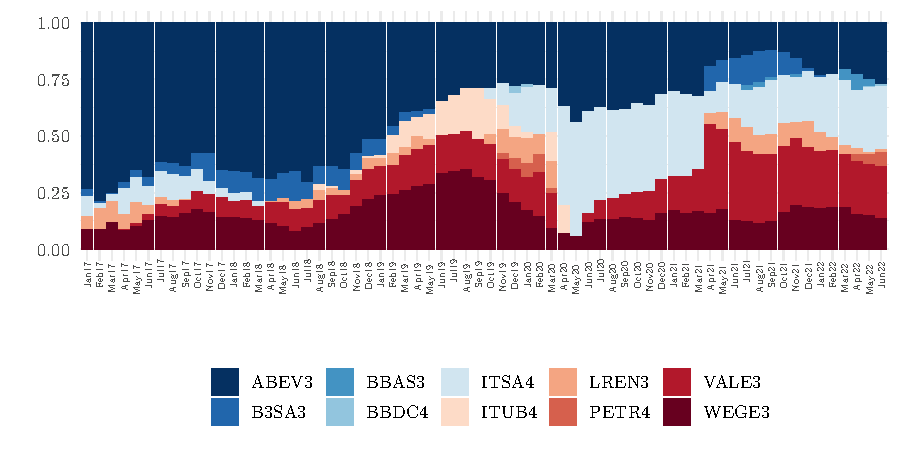
\includegraphics{figures/totalWeigthMVP.pdf}}
		\subfigure[Risks]{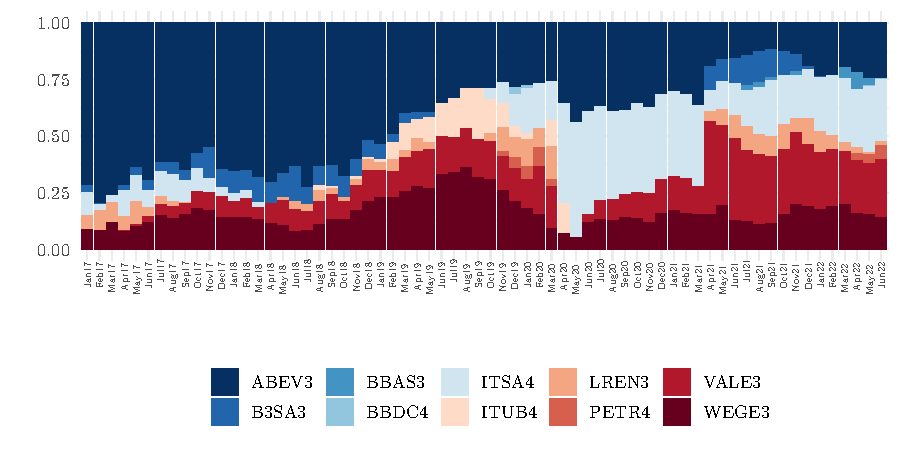
\includegraphics{figures/totalRiskMVP.pdf}}
	\end{subfigmatrix}
	\caption{Monthly distribution of MVP.}
	\label{fig:totalRiskMVP}
	%\end{adjustwidth}
\end{figure}


A RPP has the weights distributed with the purpose of having a uniform risk distribution, Figure \ref{fig:totalRiskPPP} shows the distribution of weights and risks in our backtest study.

\begin{figure}[H]
	%\begin{adjustwidth}{2.2cm}{2.2cm}
	\begin{subfigmatrix}{2}
		\subfigure[Weigths]{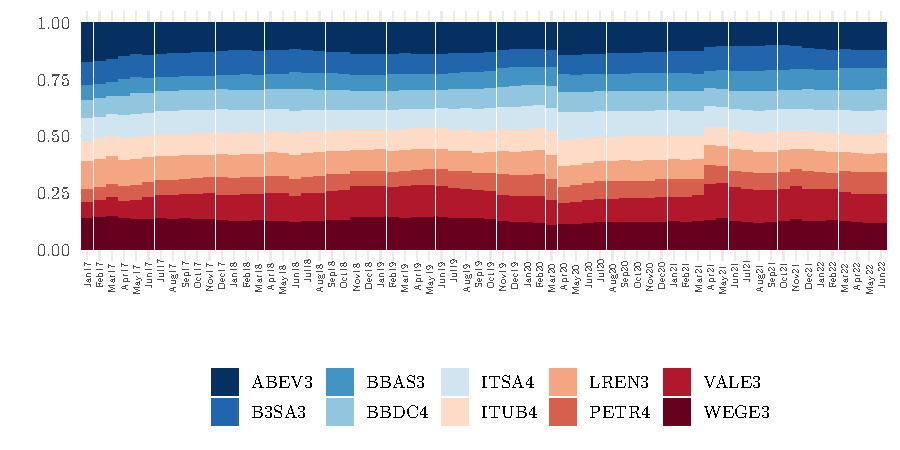
\includegraphics{figures/totalWeigthRPP.pdf}}
		\subfigure[Risks]{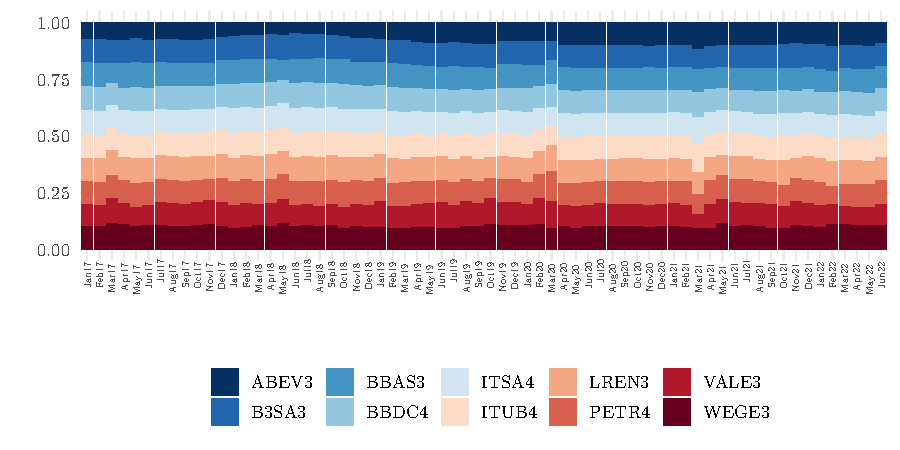
\includegraphics{figures/totalRiskRPP.pdf}}
	\end{subfigmatrix}
	\caption{Monthly distribution of RPP.}
	\label{fig:totalRiskPPP}
	%\end{adjustwidth}
\end{figure}

The total return of the RPP was greater than the MVP in the period studied. While MVP had a total return of 52\%, the accumulated RPP return was 119\% (44\% higher than the MVP).

\begin{figure}[H]
	\centering
	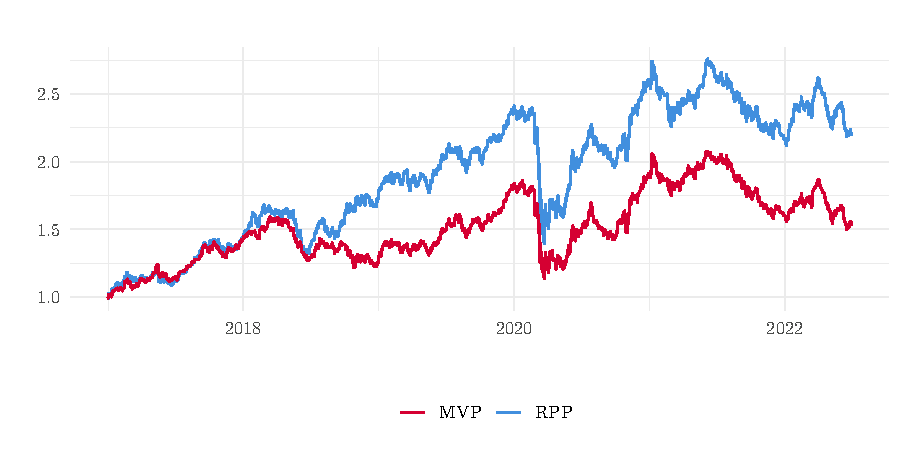
\includegraphics{figures/retornoRPPMVP.pdf}
	\caption{MVP and RPP accumulated returns: January 2017 $-$ June 2022.}
	\label{fig:retornoRPPMVP}
\end{figure}

The MVP volatility was slightly smaller than the RPP. However, considering the zero risk-free rate, the RRP Sharpe ratio was bigger than the MVP.

\begin{table}[!htb]
    \centering
      \begingroup
      \fontsize{9}{9}
      \selectfont 
\begin{tabular}{>{}lrr}
\toprule
  & MVP & RPP\\
\midrule
\textbf{Annualized Return} & 0.0785 & 0.1505\\
\textbf{Annualized Std Dev} & 0.2419 & 0.2637\\
\textbf{Annualized Sharpe (Rf=0\%)} & 0.3246 & 0.5708\\
\bottomrule
\end{tabular} \caption{Annualized returns: January 2017 - June 2022.}
      \label{tab:RPP}  % LEMBRE-SE DE MUDAR O LABEL
      \endgroup{}
      \end{table}


We remind that after 2020, due to the COVID-19 pandemic, the volatility of all assets has exploded, so we separate two period in our study, from 2017 until 2019 and after 2020. We may observe that the RPP performed much better (135\% gain) than the MVP (79\% gain) in the period between January 2017 and December 2019. Besides, MVP had a great annualized Sharpe ratio of 1.20, however, lower than RPP annualized Sharpe ratio (1.58). 

\begin{table}[!htb]
	\centering
	\begingroup
	\fontsize{9}{9}
	\selectfont
	\begin{tabular}{>{}lrr}
		\toprule
		                                    & MVP    & RPP    \\
		\midrule
		\textbf{Annualized Return}          & 0.2107 & 0.3212 \\
		\textbf{Annualized Std Dev}         & 0.1744 & 0.2027 \\
		\textbf{Annualized Sharpe (Rf=0\%)} & 1.2087 & 1.5851 \\
		\bottomrule
	\end{tabular} \caption{Annualized returns: January 2017 - December 2019.}
	\label{tab:RPP1}  % LEMBRE-SE DE MUDAR O LABEL
	\endgroup{}
\end{table}

\begin{figure}[H]
	%\begin{adjustwidth}{2.2cm}{2.2cm}
	\begin{subfigmatrix}{2}
		\subfigure[January 2017 $-$ December 2019.]{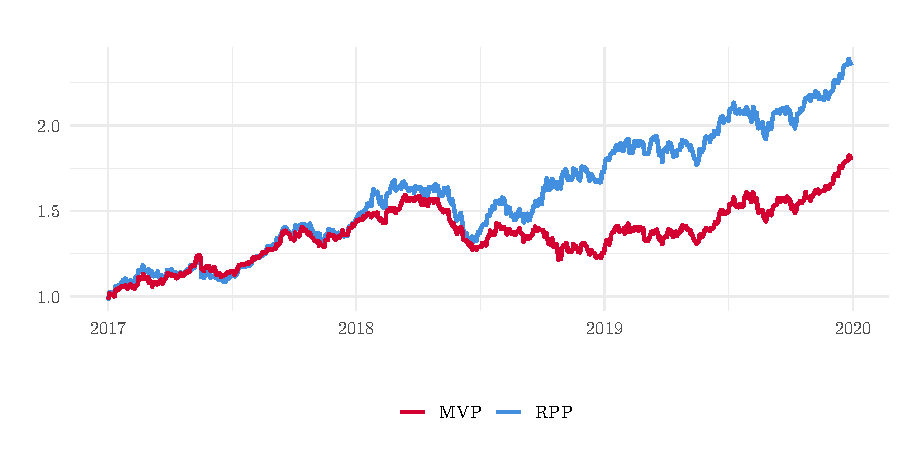
\includegraphics{figures/retornoRPPMVP1.pdf}}
		\subfigure[January 2020 $-$ June 2022.]{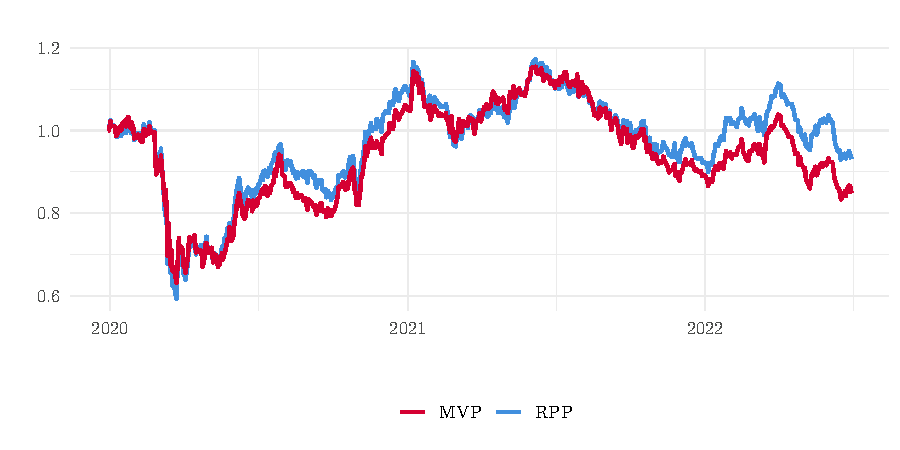
\includegraphics{figures/retornoRPPMVP2.pdf}}
	\end{subfigmatrix}
	\caption{MVP and RPP accumulated returns.}
	\label{fig:retornoRPPMVP12}
	%\end{adjustwidth}
\end{figure}

From January 2020 to June 2022, MVP exhibited an accumulated $15.2\%$ loss, while RPP reduced the loss to only $6.8\%$. Despite the loss in the period, the RPP improved the protection of the invested capital.

\begin{table}[!htb]
    \centering
      \begingroup
\fontsize{9}{9}
\selectfont
\begin{tabular}{>{}lrr}
	\toprule
	                                    & MVP     & RPP     \\
	\midrule
	\textbf{Annualized Return}          & -0.0631 & -0.0278 \\
	\textbf{Annualized Std Dev}         & 0.3046  & 0.3227  \\
	\textbf{Annualized Sharpe (Rf=0\%)} & -0.2070 & -0.0860 \\
	\bottomrule
\end{tabular}
\caption{Annualized returns: January 2020 - June 2022.}
\label{tab:RPP2}  % LEMBRE-SE DE MUDAR O LABEL
\endgroup{}
\end{table}

In our study, the RPP had a superior performance when compared to the MVP, both in high and low moments. Clearly, this study is not conclusive, but simply an example of the use of Algorithm~\ref{Alg:GeneralSeach}.

